%%%%%%%%%%%%%%%%%%%%%%%%%%%%%%%%%%%%%%%%%%%%%%%%%
\section{Data Sample and Basic Reconstruction}
%%%%%%%%%%%%%%%%%%%%%%%%%%%%%%%%%%%%%%%%%%%%%%%%%%
\subsection{Collected Data}
Table~\ref{Table:Data} shows list of the collected data while Oct/2010 Run.
800 MeV/$c$ $\pi^+$ is expected to pass-through the detector as almost minimum ionizing,
and have uniform energy deposition to all the TPC channels.
So this data set is useful for calibrating the detector response (See Sec.~\ref{Sec:Pion}).
800 MeV/$c$ proton stops after ~15 cm of flight distance inside the TPC fiducial volume
with relatively large $dE/dx$. So we use the proton data set for validation of the
detector response at high $dE/dx$ region(See Sec.~\ref{Sec:Proton}).
We have collected three different $K^+$ data by varying thickness of the degrader. 
540, 630, 680 MeV/$c$ correspond to the momentum degraded by 
2 lead glass, 1 lead glass + 1 lead block, and 1 lead glass, respectively, 
and such $K^+$ stops after 10 cm, 50 cm, and 65 cm of flight distance inside TPC fiducial volume.

\begin{table}[h]
\begin{center}
\caption{List of collected data}
\begin{tabular}{l|ll}
  Particle  &Initial Momentum (MeV/$c$) &Number of Events\\
\hline
  Pion      &800                &3,000\\
  Proton    &800                &1,500\\
  Kaon      &540 (2LG)          &7,000\\
  Kaon      &630 (1LG+1LB)      &40,000\\
  Kaon      &680 (1LB)          &35,000\\
  electron  &800                &2,500\\
  electron  &200                &10,000\\
  pion      &200                &10,000\\
\end{tabular}
\label{Table:Data}
\end{center}
\end{table}

Top plot in Fig.~\ref{Fig:Textbook} shows 2D display of an event taken with 800 MeV/$c$ electron trigger.
Horizontal axis corresponds to TPC channel number where zero means most upper stream strip. 
Since strip pitch is 1 cm, this is equivalent to distance from beam injection point in cm.
Vertical axis corresponds to electron drift time in $\mu$s
where t=0 means trigger timing. 
In 250L TPC, anode and cathode is located at top and bottom of the detector, respectively,
drift direction is from bottom to top of the detector.
With 200 V/cm of electric field, drift velocity is about 0.8 m/ms,
and drift time of full detector (40 cm) is about 500 $\mu$s.
Color strength of the plot corresponds to the TPC signal pulse height in ADC counts.
In this event, triggered electron can be clearly identified in the center of the detector
as an electromagnetic shower,  while there are two other particles 
accidentally overlapped with the triggered electron. 
Track at t=100 $\mu$s is considered as
a proton which stops after 15 cm of flight distance and 
has large $dE/dx$ around the stopped point.
Track at t=400 $\mu$s is considered as
a pion which passes-through the detector and 
has uniform $dE/dx$ over the TPC channels.
Bottom plot in Fig.~\ref{Fig:Textbook} shows a typical $K^+ \to\mu^+\nu$ like event.
We can clearly identify a kink of the track at 60 cm which is considered
as stopped point of Kaon and it decays to $\mu^+\nu$ .
Energy deposition of the track is about MIP at the injection point
and gradually increase towards the stopped point at 60 cm.

\begin{figure}[htbp]
 \begin{center}
  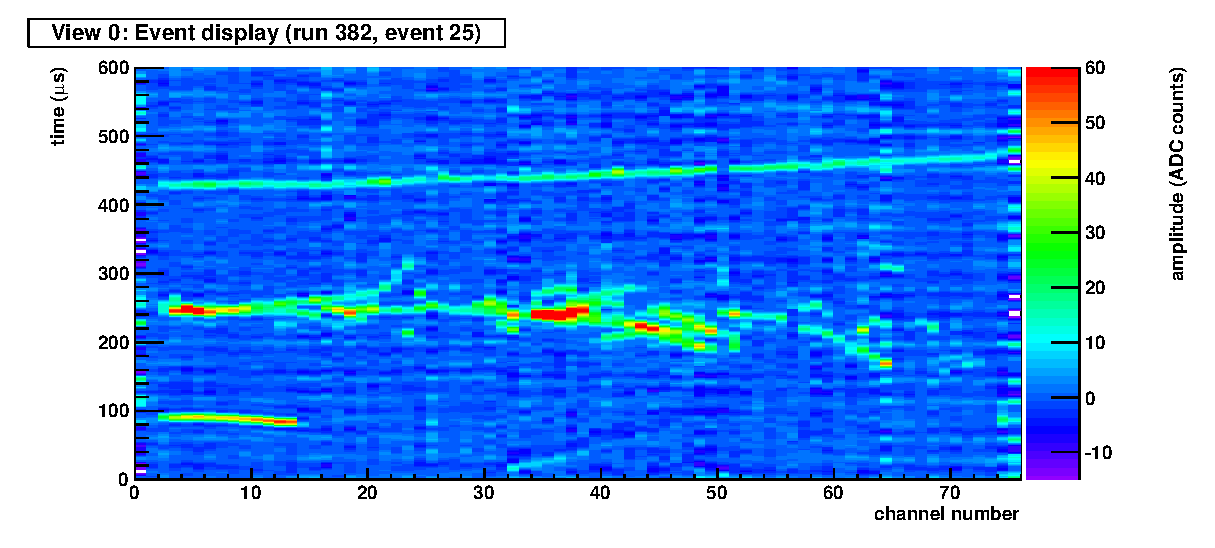
\includegraphics[width=1.0\hsize]{fig/Textbook.eps}
  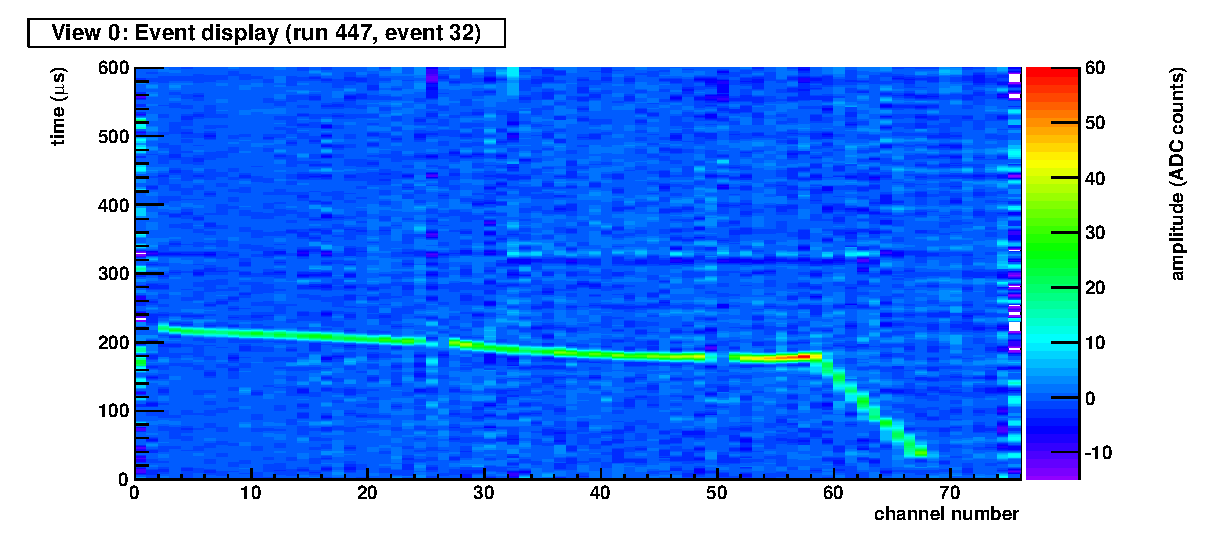
\includegraphics[width=1.0\hsize]{fig/Kmunu.eps}
 \end{center}
 \caption{Event display of 800 MeV/$c$ electron triggered event (top) accidentally overlapped with a proton and a pion,
   and Kaon 630 MeV/$c$ triggered event (bottom)}
 \label{Fig:Textbook}
\end{figure}


\subsection{Noise Reduction}
Dotted line in top plots of Fig.~\ref{Fig:FFT} shows raw waveform of the TPC signal
before applying any noise reduction. the waveform shown in this plot
are channel 13 in Fig.~\ref{Fig:Textbook} which are around the proton stopped point.
Signal-to-noise ratio for this particular case is poor and pion signal 
which is supposed to be t=400 $\mu$s is almost hidden by the noise. 
While time width of TPC signal is few $\mu$s which is determined by
drift time between anode and anode-grid, dominant noise component looks
higher frequency. To reduce such noises, we have applied FFT 
(Fast Flourier Transformation) filter to cut the high frequency component.
Bottom plot in Fig.~\ref{Fig:FFT} shows amplitude as a function of frequency
for the same event. This clearly shows dominant noise component with
$>$ 200 kHz has good separation with signal component ($<$ 100 kHz).
Solid line in top plot of Fig.~\ref{Fig:FFT} shows waveform after removing high frequency
($>$ 80 kHz) component by the FFT filter. Signal-to-noise ratio is dramatically
improved. On the other hand, we expect certain bias to the signal charge
measurement by this filter, and it will be discussed in Section x.

\begin{figure}[htbp]
 \begin{center}
  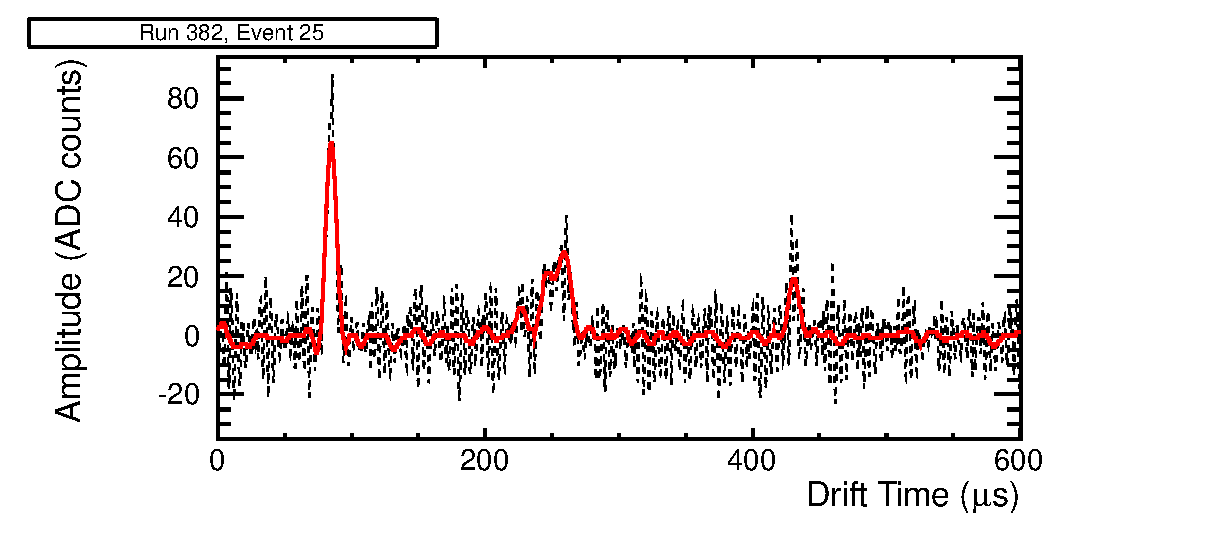
\includegraphics[width=1.0\hsize]{fig/beforeafterFFT.eps}
  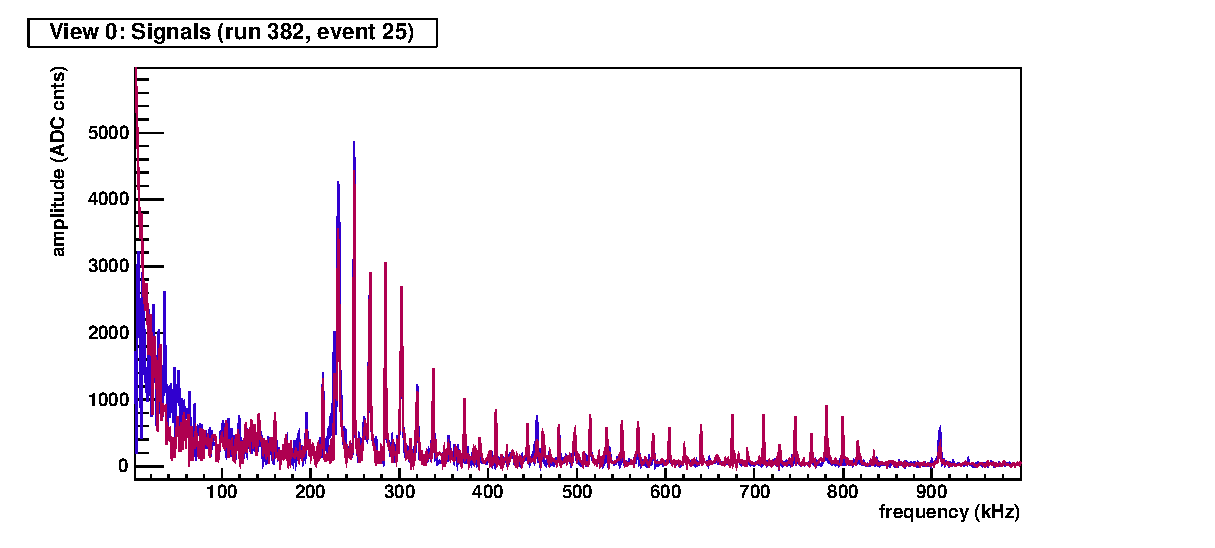
\includegraphics[width=1.0\hsize]{fig/FFT.eps}
 \end{center}
 \caption{Top: Typical TPC signal waveform before (dotted line) and after (solid line) applying FFT low pass filter with threshold of 80 kHz,
Bottom: FFT frequency amplitude distribution}
 \label{Fig:FFT}
\end{figure}

\subsection{Hit Finding/Clustering}
After noise reduction we find signal hits and create clusters associated to single tracks. 
Hit is defined as bump over given threshold in a channel. 
Threshold of hit finding is 6 ADC counts, which is about 2.5$\sigma$ from typical data noise 
level (as shown in Fig~\ref{Fig:FFT}) and keeping more than 99\% of Kaon hit finding efficiency in simulation.
% noise level from outside window of PhysicsOct55 (rms~2.49)
ADC count distribution is fitted by Gaussian plus step function to estimate the charge of hit in ADC $\times$ $\mu$s unit.
Fitting $\chi^2 < 3$ and $2.5<$~(time~width~of~hit)~$<8$~$\mu$s are required to remove noise hits further.
After finding all hits in an event, we construct cluster by merging adjacent hits. 
The example of hit finding and clustering using Fig~\ref{Fig:Textbook} event is shown in Fig~\ref{fig:Clustering}, which indicates reasonable hit and cluster findings. 

\begin{figure}[htbp]
 \begin{center}
  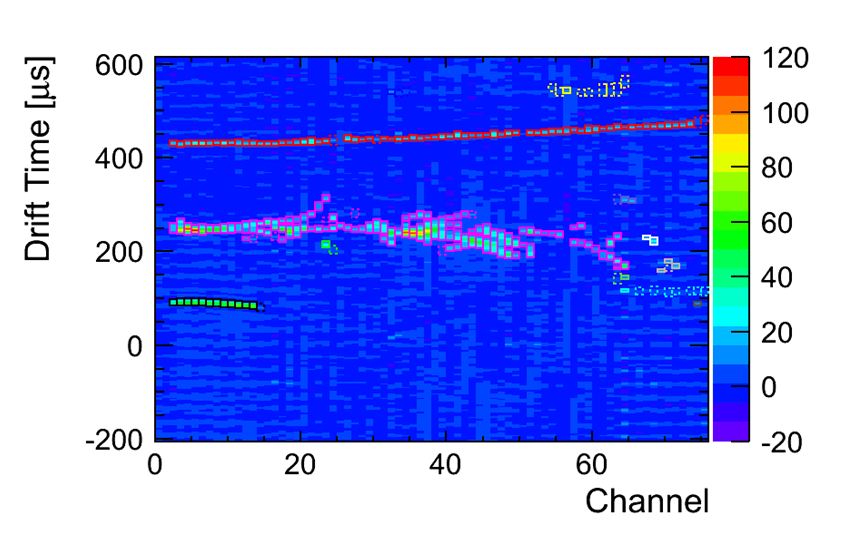
\includegraphics[width=1.0\hsize]{fig/clustering.eps}
 \end{center}
 \caption{Example of hit finding and clustering. A colored box corresponds to a hit and colors represent different clusters.}
 \label{fig:Clustering}
\end{figure}


